\section{Privacy Via Chameleon}
The results in the previous section demonstrate the huge utility loss in the perturbed representative instance after adding noise to provide privacy guarantee. In this section, we propose a novel uncertainty-aware algorithm called Chameleon that enables uncertainty-aware control over the noise injected into the \emph{original uncertain} graph. This qualifies Chameleon to provide enough privacy guarantee in better utility. 

\subsection{The Chameleon framework}
\begin{algorithm}
{\scriptsize
	\begin{algorithmic}[1]
    	\item[] {\textbf{Input:}~Graph $\mathcal{G}$, obfuscation level $k$, tolerance parameter $\epsilon$}
        \item[] {\textbf{Output:}~The result $\mathcal{G}_{obf}$}
     	\STATE {$\sigma_{l} \leftarrow 0$; $\sigma_{u} \leftarrow 1$} \\
        \REPEAT
        \STATE{$\langle \hat{\epsilon}, \hat{\mathcal{G}} \rangle$ $\leftarrow$ \textbf{genObf}(-,$\sigma_{u}$)} \\
        \STATE{{\bf if} $\hat{\epsilon}=1$ (fail) {\bf then} $\sigma_{l} \leftarrow \sigma_{u}$; $\sigma_{u} \leftarrow 2\sigma_{u}$}
        \UNTIL{$\hat{\epsilon} \neq 1 $} \\
        \REPEAT
        	\STATE {$\sigma_{mid} \leftarrow (\sigma_{u}+\sigma_{l})/2$}
            \STATE{$\langle \hat{\epsilon}, \hat{\mathcal{G}} \rangle$ $\leftarrow$ \textbf{genObf}(-,$\sigma_{mid}$)}
            \STATE {{\bf if} $\hat{\epsilon} =1$~{\bf then}~$\sigma_{l} \leftarrow \sigma_{mid}$}\\
            \STATE {{\bf else} $\sigma_{u} \leftarrow \sigma_{mid}$;~~{$\mathcal{G}}_{obf} \leftarrow \hat{\mathcal{G}}$}
        \UNTIL{$\sigma_{u}-\sigma_{l}$ is enough small}
        % \COMMENT{\textcolor{blue}{\scriptsize Binary search for better obfuscation}}
        \STATE {return $\mathcal{G}_{obf}$}
    	\caption{The obfuscation algorithm}
	 \label{alg:obf}
    \end{algorithmic}
    }
\end{algorithm}
\vspace{-7pt}

We now introduce the state-of-art perturbation algorithm~\cite{Boldi_Injecting_2012} that computes the noise needed to injected into the input \emph{determinitic} graph to obtain the desired privacy level. Each selected edge is altered based on a stochastic variable drawn from a trunated Normal distribution, $R(\sigma)$. This distribution has density function proportional to the Normal distribution, with mean $0$ and variance $\sigma^2$. Thus, small values of $\sigma$ contribute towards better utility, but at the same time they provide lower level of obfuscation. Targeting for high utility, the algorithm aims at injecting the minmal amount of noise need to achieve the required obfuscation. Its computation is achieved via a binary search on the value of the noise uncertainty parameter $\sigma$, as shown in Algorithm~\ref{}. 
% change a litte 

The core function of this process is the \texttt{GenObf} function which performs following core steps:
\begin{itemize}
    \item{Select a subset of edges subjects to further alteration;}
    \item{Alter selected edges as the computed amount of noise;}
\end{itemize}

\textbf{Contribution}~~The conventional schemes are plausible if the operating edge probability is binary, which is unreasonable when dealing with uncertain graphs. Our goal is to develop a privacy mechanism that reduced the amount of noise that must be added to achieve a given privacy level for \emph{uncertain} graphs. Our insight is to shift an existing framework for anonymizing \emph{probabilistic} graphs by integrating uncertainty semantics into two core steps. 

\subsection{Uncertainty-aware Edge Selection}
Figuring out the optimal subset of edges that balances the privacy gain and the utility loss is a typical combinational optimization problem. It involves the consideration over the exponential number of edge combinations. Let alone the infinite possibilities of probability values on the selected edges, which further complicates the problem.

To alleviate combinational intractability, the heuristics that have been proposed so far for anonymizing deterministic graphs can be classified into two main categories: 
(1)~{\em Anonymity-oriented} heuristics that suggest injecting larger perturbations to the edges associated with the less-anonymized (more-unique) 
nodes~\cite{Boldi_Injecting_2012,Ying2009,Liu_Towards_2008, Thompson_The_2009,Zhou_Preserving_2008,casasprivacy,Ying_Randomizing_2008,Wang2011,Das_Anonymizing_2010,Wu_k_2010,Liu_Privacy_2009,Ninggal_Utility_2015}, and 
(2)~{\em Utility-oriented} heuristics that suggest avoiding perturbations over {\em ``bridge"} and sensitive edges whose deletion or addition would 
significantly impact the graph structure~\cite{casasprivacy,Ying_Randomizing_2008,Wang2011,Das_Anonymizing_2010,Wu_k_2010,Liu_Privacy_2009,Ninggal_Utility_2015}.
Note that these two types are complementary to each other and combining them would introduce an added benefit as confirmed by practice in deterministic graph anonymization~\cite{casasprivacy}. Nevertheless, these two types of heuristics and their combination have not been explored yet in the context of \emph{uncertain} graphs.

In this paper, we first extend the idea of \emph{uniqueness} score via density estimation. Second, we propose a novel edge relevance that extends well-known graph concepts, such as ``cut edge" for estimating structural errors incurred by edge probability alterations. In order to compute edge relevance in \emph{uncertain} graphs, we design an algorithm based sampling. Finally, we utilize these \emph{uncertainty}-embedded metaheuristics to effectively selecting edges for further alteration. 

\subsection{Uniqueness Score}
Intutively, larger amount of noise should be added at nodes that are less anonymized (i.e, more distinctive) in the original graphs. \emph{Uniqueness score} is shown to be an effective metric of how typical is the node $v$ among the nodes of the graph~\cite{Boldi_Injecting_2012}. The formal defintion of uniqueness score is given as follows. 
\begin{definition}
    \textbf{Uniqueness Score~\cite{Boldi_Injecting_2012}}
     Let $P:V \rightarrow  \Omega_{P}$ be a property on the set of nodes $V$ of the graph $\mathcal{G}$, let $d$ be a distance function on $\Omega_{P}$, and let $\theta >0$  be a parameter. 
  Then the $\theta-commonness$ of the property values $\omega \in \Omega_{P}$ is $C_{\theta}(\omega):= \sum_{u \in V} \Phi_{0,\theta}(d(\omega, P(v)))$,   
while the $\theta$-uniqueness of $\omega \in \Omega_{P}$ is $U_{\theta}:= \frac{1}{C_{\theta}(\omega)}$. 
\end{definition} 

Note that, it adopts a parametric way to estimate the probability density function of the property value $\omega$ (i.e., how typical the value is among all the nodes). For the density estimate, we place a normal kernel with standard variance 
$\theta$ which implies the spread out of the property value over the domain. In the previous work~\cite{Boldi_Injecting_2012}, they set $\theta=\sigma$, where $\sigma$ is the standard deviation of the noise generation Gaussian distribution. This is because the larger injected amount of uncertainties indicates that the property values may be spread out in a larger domain. 

Here, we set $\theta$ equals $\sigma_{\mathcal{G}}$ as the latter represents the spread of property value in the \emph{uncertain graph}. For a given node with the property $\omega$, we can compute its ``uniqueness" score as the reverse of its density. The higher the uniqueness score the less-protected the node and the more anonymization it eventually needs.

\subsection{Reliability Relevance}

\textbf{\emph{Observation}}~~Namely, alteration over any single uncertain edges (partial added or deleted) would produce structural changes that send ripples through the rest of the graph. 
The same amount of alteration performed over different edges may incur significantly different structure change. 
Referring to the example in Figure~\ref{fig:edgeRRGraph}, two vertices $\tt{a}$ and $\tt{e}$ will be assigned the same {\em uniqueness score} due to the exact probabilities associated with their edges. 
As a result, the {\em anonymity-oriented} strategy would select and perturb either of the two edges $(\tt{a},\tt{c})$ and $(\tt{c},\tt{e})$ with the same probability. However, the modifications to $(\tt{c},\tt{e})$---which is the only link between two~\emph{reliable} clusters---clearly incurs much larger structure distortion than that on $(\tt{a},\tt{c})$. To control the utility loss, it is cruical to quantify the structural impact of a single edge alteration by any granularity. 



\textbf{Contribution.}~~To this end, we propose a theoretically sound estimation for the {\em ``reliability deviation''} caused by individual uncertain edge modifications in a fine-grained way. 
Following this path, we introduce a new measure, called {\em Edge Reliability Relevance $(\mathcal{E}RR)$}, at the edge level, and an aggregated measure, called {\em Vertex Reliability Relevance} $(\mathcal{V}RR)$, at the vertex level as will be formally defined next. These measures will enable ranking the edges to be targeted for obfuscation in a meaningful utility-based perspective. Besides, we provide an algorithm for computing them efficiently. 


\begin{figure}
  \vspace{-1em}
    %\captionsetup{justification=centering,margin=0cm}
  \subfigure[An uncertain graph]{\label{fig:edgeRRGraph}  %(22)
    \begin{minipage}[l]{0.45\columnwidth}
      \centering
      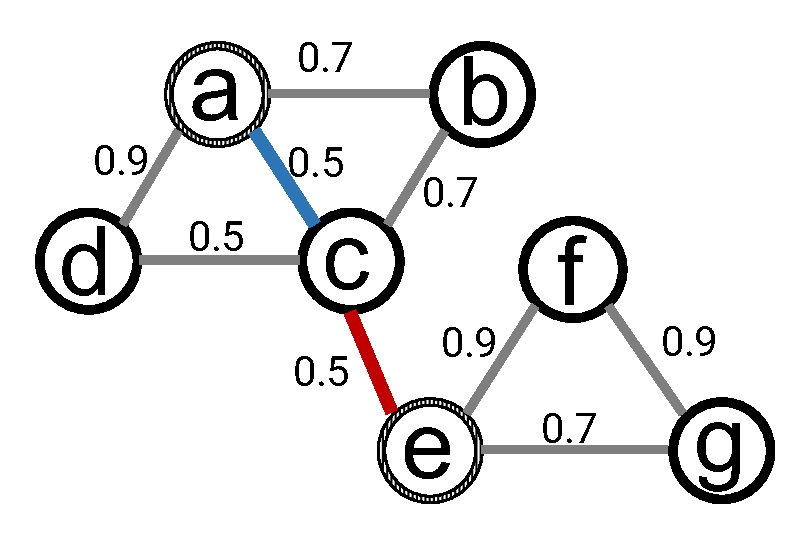
\includegraphics[height=3cm]{AddFigure/bridgetExample.pdf}
    \end{minipage}
  }
  \subfigure[The reliability $R_{a,e}$ v.s $p(e)$]{\label{fig:edgeRR}  %(22)
    \begin{minipage}[l]{0.5\columnwidth}
      \centering
      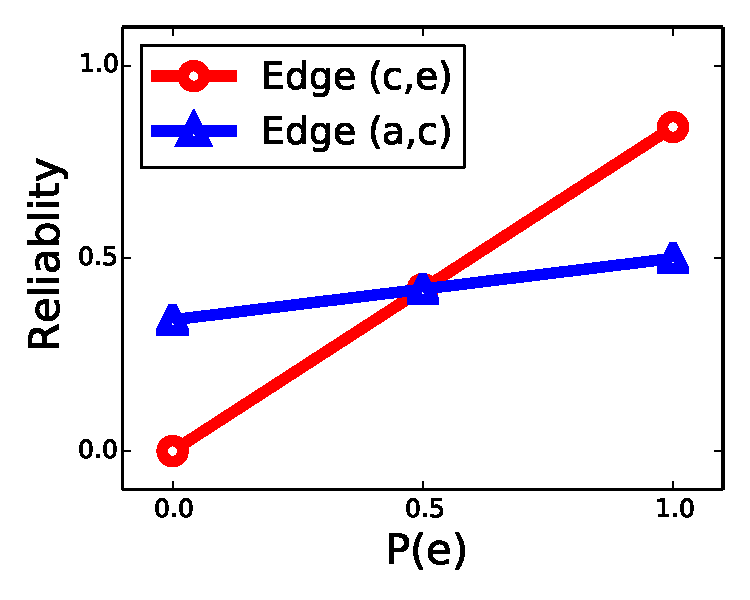
\includegraphics[height=3cm]{AddFigure/ErrExample.pdf}
    \end{minipage}
  }
    \vspace{-1em}
    \caption{(a) Different edges have different effect on the overall graph reliability. (b) Formal {\em Reliability Relevance } measure. A bigger edge's slope indicates  
     big distortion in reliability under small changes to the edge's probability.}
    \vspace{-15pt}
\end{figure}


\textbf{Edge Relevance Analysis.}~~In the context of uncertain graphs, the reliability relevance of edge is defined as reliability discrepancy when one single edge is alterred. Changing a single edge in $\mathcal{G}$ will result in one or more point-wise reliability changing in the corresponding \emph{uncertain} graphs. Thus, the edge reliability relevance is computed as the sum of reliability deviation caused by a single edge alteration. 

\begin{definition} 
  \textbf{Single Edge Reliability Relevance.}~~Given an uncertain graph, the sensitivity of two-terminal reliability $R_{u,v}$ over edge $e$ is defined as follows:
  \begin{align*}
    \mathcal{E}RR^{e}_{u,v} = \lim_{h \rightarrow 0 } \frac{R_{u,v}(\mathcal{G'})-R_{u,v}(\mathcal{G})}{h}
  \end{align*}
  where $\mathcal{G'}$ are identical to the original graph expect the edge $e$ with modified probability $p(e)+h$.
\end{definition}


\begin{lemma}
    \textbf{Factorization Lemma}~~Given an uncertain graph $\mathcal{G}$, the reliability of the node pair $(u,v)$, i.e., $R_{u,v}(\mathcal{G})$, can be factorized via a specific uncertain edge $e$ as follows:
    % \begin{equation*}
    \begin{align*}
      R_{u,v}(\mathcal{G}) &= p(e) R_{u,v} (\mathcal{G}_{e}) + (1-p(e)) R_{u,v} (\mathcal{G}_{\bar{e}}) \\
                          & = p(e) \big[ R_{u,v} (\mathcal{G}_{e}) - R_{u,v} (\mathcal{G}_{\bar{e}}) \big] + R_{u,v} (\mathcal{G}_{\bar{e}})
    \end{align*}
    where uncertain graphs $\mathcal{G}_{e}$ and  $\mathcal{G}_{\bar{e}}$ are identical to the original graph $\mathcal{G}$ with the 
    exception that $e$ is certainly present in the former and certainly not present in the later.
    \label{lemma:fac} 
\end{lemma}

Lemma~\ref{lemma:fac} indicates that the \emph{deviation} of $R_{u,v}$ introduced by a specific edge $e$ is \emph{linear} to the amount of edge probability deviation as shown in Figure~\ref{fig:edgeRR}. In other words, the edge reliability relevance $\mathcal{E}RR^{e}_{u,v}$ equals to the difference of $R_{u,v}$ in the corresponding neighbor \emph{uncertain graphs} $\mathcal{G}_{e}$ and $\mathcal{G}_{\bar{e}}$. First, we remind the reader that edge reliability relevance always be positive since all the connected pairs in $\mathcal{G}_{e}$ are guaranteed to be a superset or at least equal to that in $\mathcal{G}_{\bar{e}}$.


By aggregating edge relevance among all the node pairs $\langle u,v \rangle$, we can get the overall {\em reliability relevance} of edge $e$ $\mathcal{E}RR^{e}(\mathcal{G})$ defined as 
\begin{align*}
    \vspace{-1em}
    \mathcal{E}RR^e(\mathcal{G}) &= \sum_{u,v} |\mathcal{E}RR^e_{u,v}(\mathcal{G})| \\
                                 &= \sum_{u,v} |R_{u,v}(\mathcal{G}_{e}) -R_{u,v}(\mathcal{G}_{\bar{e}})| \\  
                                 &= \sum_{u,v} R_{u,v} (\mathcal{G}_{e}) - \sum_{u,v} R_{u,v}(\mathcal{G}_{\bar{e}}) 
\end{align*}
% \vspace{-0.5em}
Note that $\mathcal{E}RR^e$ equals to the difference of the expected number of connected pairs between two uncertain graphs $\mathcal{G}_{e}$ and $\mathcal{G}_{\bar{e}}$.  
In the context of edge relevance, reliability relevance can be seen as generalization of cut-edges, which quantifies the impact of partial edge deletion or addition on the connectivity in the uncertain graph. 
When the perturbation hits those edges with higher reliability relevance, it would produce bigger structural distortion over the overall \emph{uncertain} graph. 


On the basis of these edge-level reliablity relevance, we can now compute a vertex-level reliability relevance of a given vertex (Say $u$) as a weighted sum of reliability relevance of $u$'s edges $\mathtt{E}^{u}$.  
Fix $u \in \mathcal{G}$ and let $\mathtt{E}^{u}$ be the pairs of vertices that include $v$, we have 
\begin{equation*}
    \vspace{-0.5em}
    \mathcal{V}RR^{u}(\mathcal{G})=\sum_{e \in \mathtt{E}^{u}} p(e)  \mathcal{E}RR^{e}(\mathcal{G})
    \vspace{0.5em}
\end{equation*}

The $\mathcal{V}RR^{u}(\mathcal{G})$  is a measure of the expected impact of vertex modification on the graph reliability. Namely, the higher the vertex's reliability relevance, the larger reliability distortion introduced by modification associated with its edges.



% \subsection{Reliability Relevance}

% \textbf{\emph{Observation}} As exemplified in Figure~\ref{fig:edgeRR}, each edge modification will have \emph{varying} impact to the graph structure in the context of uncertain graphs. From the perspective of \emph{uniqueness}, nodes $a$ and $e$ are identical since adjacent edges have identical uncertainties. Accordingly, anonymity-oriented heuristics would select and perturb edges $(a,b)$ and $(b,e)$ without bias. While, the deletion of the uncertain edge $(b,e)$, the only link between two \emph{reliable} clusters, clearly incurs much larger structure distortion than the deletion of the edge $(a,b)$. This observation calls for an effective measure of edge influence in the context of uncertain graphs. 

% In this work, we provide a compact analytic form of reliability deviation caused by individual uncertain edge modification in a fine-grained way, namely edge probability alteration in any granularity. Following this path, we introduce the concept of edge reliability relevance, which equals the sum expectation of reliability discrepancy of all the node pairs. Besides, we provide an algorithm for computing edge \emph{reliability relevance} (RR) efficiently. 

